\documentclass[10pt,a4paper]{article}

\usepackage[
	top=3.05cm,
	bottom=4.2cm,
	left=2.6cm,
	right=2.6cm
]{geometry}
\usepackage{fontspec}
\usepackage{graphicx}
\usepackage{multicol}
\usepackage{titlesec}
\usepackage{hyperref}
\usepackage[english]{babel}

\setmainfont{Arial}
\pagestyle{empty}
\setlength{\parindent}{0pt}
\setlength{\parskip}{0.40em}
\setlength{\columnsep}{0.8cm}
\setlength{\emergencystretch}{2em}
\hypersetup{hidelinks}

\titleformat{\section}
	{\normalfont\bfseries\fontsize{10}{12}\selectfont}
	{}
	{0pt}
	{}
\titlespacing*{\section}{0pt}{0.68em}{0.25em}

\begin{document}

\noindent
\includegraphics[width=2.05cm]{assets/siicusp34-logo-en.png}

\begin{center}
	\vspace{0.15em}
	{\bfseries\fontsize{14}{16}\selectfont EXACT ALGORITHMS FOR THE TOURING POLYGONS PROBLEM\par}
	\vspace{0.30em}
	{\fontsize{11}{13}\selectfont Gabriel Freire Ushijima\textsuperscript{1}\par}
	{\fontsize{11}{13}\selectfont Ernesto G. Birgin\textsuperscript{2} - Advisor\par}
	{\fontsize{11}{13}\selectfont IME-USP\par}
	{\fontsize{10}{12}\selectfont \textsuperscript{1}\href{mailto:gabriel_ushijima@usp.br}{gabriel\_ushijima@usp.br} \quad \textsuperscript{2}\href{mailto:egbirgin@ime.usp.br}{egbirgin@ime.usp.br}\par}
\end{center}

\begin{multicols}{2}

\section{Objectives}

The Touring Polygons Problem (TPP) asks for a shortest Euclidean path that starts at a point \(s\), visits a sequence of polygons \(P_1,\ldots,P_k\) in the plane, and ends at a point \(t\). The path does not have to visit predefined points: it is enough to touch the boundary or pass through each region. This makes the problem suitable for settings in which targets are areas rather than points, such as urban delivery zones, sensor or radio coverage, pickup, inspection, and autonomous vehicle routing. In such settings, physical obstacles and geographic constraints naturally lead to irregular non-convex regions.

This work aims to develop exact algorithms for the TPP with non-convex polygons and fixed visiting order. This variant is already NP-hard [1], but it contains an important structural subproblem: when the polygons are convex, the TPP admits a polynomial-time solution based on last-step maps. The proposed approach exploits this complexity gap by using an exact and efficient geometric solver for the convex case as the core component of a combinatorial search for the non-convex case. The same structure also prepares an ongoing extension to the free-order variant, which is closer to the Traveling Salesman Problem with Neighborhoods.

\columnbreak

\section{Materials and Methods}

The development was organized in two layers. In the first one, we implemented exact algorithms for the convex TPP. The theoretical basis is the algorithm of Dror, Efrat, Lubiw, and Mitchell [1], which constructs, for each polygon, a first-contact region and a last-step map. These maps partition the plane according to the form of the last segment of the optimal path: arrival through a vertex, arrival through an edge, or pass-through of the polygon. From these maps, the optimal path is reconstructed through successive queries, moving backward from \(t\) to \(s\).

We implemented the algorithm described in [1] and improved it with memoization, avoiding the computation of map regions that are never queried during path reconstruction. This modification preserves the \(O(nk\log(n/k))\) worst-case bound, where \(n\) is the total number of vertices, while reducing redundant work in the queries that are actually performed. We also implemented the \(O(nk)\) approach of Tan and Jiang [2]; on our instances, it did not outperform the map-based implementations, because its asymptotic gain did not offset the cost of the traversed data structures.

\end{multicols}

\vfill

\begin{center}
	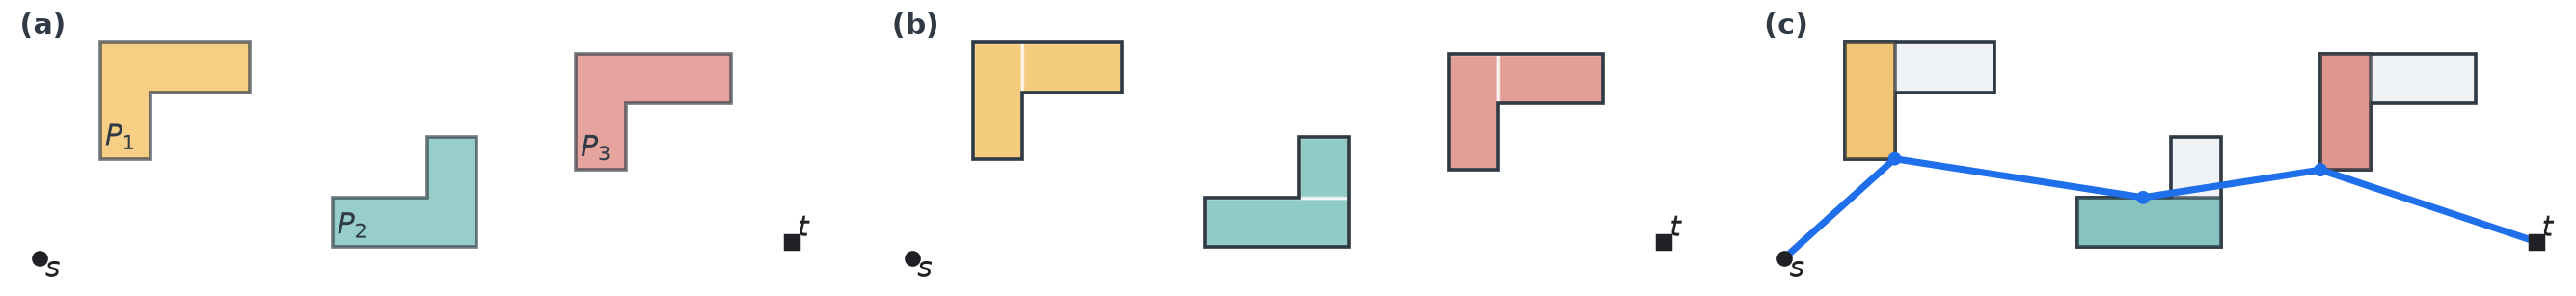
\includegraphics[width=0.96\textwidth]{assets/tpp-pipeline.pdf}\\[-0.20em]
	{\fontsize{8}{9}\selectfont Figure 1. Method pipeline: instance with non-convex regions, decomposition into convex pieces, and solution of the associated convex subproblem.}
\end{center}

\newpage

\begin{multicols}{2}

In the second layer, each non-convex polygon is decomposed into convex pieces by a self-contained implementation based on Greene's algorithm [4], validated against the corresponding CGAL routine on more than 16 thousand polygons from the test corpus. The non-convex TPP is then solved by Branch and Bound: each node fixes a partial choice of convex pieces, while the still-unfixed polygons are relaxed to their convex hulls. Solving this relaxed problem exactly gives a lower bound. If the bound exceeds the best known feasible path, the whole subtree is pruned. An initial incumbent is obtained by a discrete heuristic over representative boundary points and refined by calling the convex solver on the selected pieces.

\section{Results}

The first contribution of the work is a modular and verifiable implementation of the convex TPP, separating geometric primitives, query structures, reusable workspaces, and benchmarking tools. Experiments with synthetic instances confirm the expected asymptotic behavior and show that worst-case analysis does not fully describe the observed performance: the memoized strategy reduces redundant computations during path reconstruction, while the comparison with Tan and Jiang shows that asymptotic complexity alone does not determine practical performance.

The second contribution is the effective reduction of the fixed-order non-convex TPP to a search controlled by geometric lower bounds. Direct enumeration of piece choices is infeasible. For example, in an instance with 59 polygons, the decomposition yields a search space on the order of \(2\cdot10^{33}\) combinations. The current Branch and Bound implementation solves an instance of this scale with about 2 million calls to the convex solver, in approximately 25 seconds, indicating a reduction of many orders of magnitude in the work needed to prove optimality.

In addition, we built an experimental infrastructure that records convex solver calls, visited nodes, pruned nodes, incumbent quality, piece distributions, and time spent in each stage. An interactive visualization tool was also developed to construct instances, inspect solutions, and display last-step maps, supporting the geometric validation of the algorithms.

\section{Conclusions}

The work shows that combining computational geometry and combinatorial optimization is a promising approach for the non-convex TPP. Instead of formulating the entire problem directly in a generic solver, the proposed strategy uses an exact geometric algorithm for the convex subproblem and embeds it in a Branch and Bound tree. This yields an exact solution, reduces dependence on commercial solvers in the core method, and makes instances tractable that would be impossible to solve by direct enumeration.

Future work will strengthen the lower bounds, explore more economical convex decompositions, and extend the search tree so that it also decides the visiting order of the polygons. This extension connects the project to variants of the Traveling Salesman Problem with Neighborhoods and to exact routing models with polygonal regions.

The author declares no conflict of interest.

Supported by FAPESP grant 2025/13861-1.

\section{References}

[1] M. Dror, A. Efrat, A. Lubiw, and J. S. B. Mitchell. Touring a sequence of polygons. \textit{Proceedings of the 35th Annual ACM Symposium on Theory of Computing}, 473-482, 2003.

[2] X. Tan and B. Jiang. Efficient algorithms for touring a sequence of convex polygons and related problems. \textit{Theory and Applications of Models of Computation}, 614-627, 2017.

[3] E. M. Arkin, S. P. Fekete, and J. S. B. Mitchell. The Traveling Salesman Problem with Neighborhoods: A Survey. In \textit{The Traveling Salesman Problem and Its Variations}, Springer, 2005.

[4] D. H. Greene. The decomposition of polygons into convex parts. In F. P. Preparata, editor, \textit{Computational Geometry}, 235-259, JAI Press, 1983.

[5] I. Gentilini, F. Margot, and K. Shimada. The travelling salesman problem with neighbourhoods: MINLP solution. \textit{Optimization Methods and Software}, 28(2):364-378, 2013.

\end{multicols}

\end{document}
